\chapter{Summary of the Technical Drawings and Developed Codes}
\label{apendice2}

In this appendix, the Section~\ref{appendice:technicalDrawings} illustrates the technical drawings regarding the development of the 3D device through the SolidWorks software.

Already, for the Section~\ref{appendice:code}, it provides the link for the GitHub, where the user can find the documents developed. The files are divided as follows:

\begin{itemize}
    \item The \textit{api} file contain all the Appication Program Interface developed using PHP programming language.
    \item Already for the \textit{application} file, it gives the access to the Front End application, where can be found the HTML/CSS and JavaScript codes.
    \item In \textit{esp32\_code} file, it is found the code structure developed using Arduino IDE in C programming language.
\end{itemize}




\clearpage
\section{Technical Drawings}\label{appendice:technicalDrawings}

\begin{figure}[h!]
    \centering
    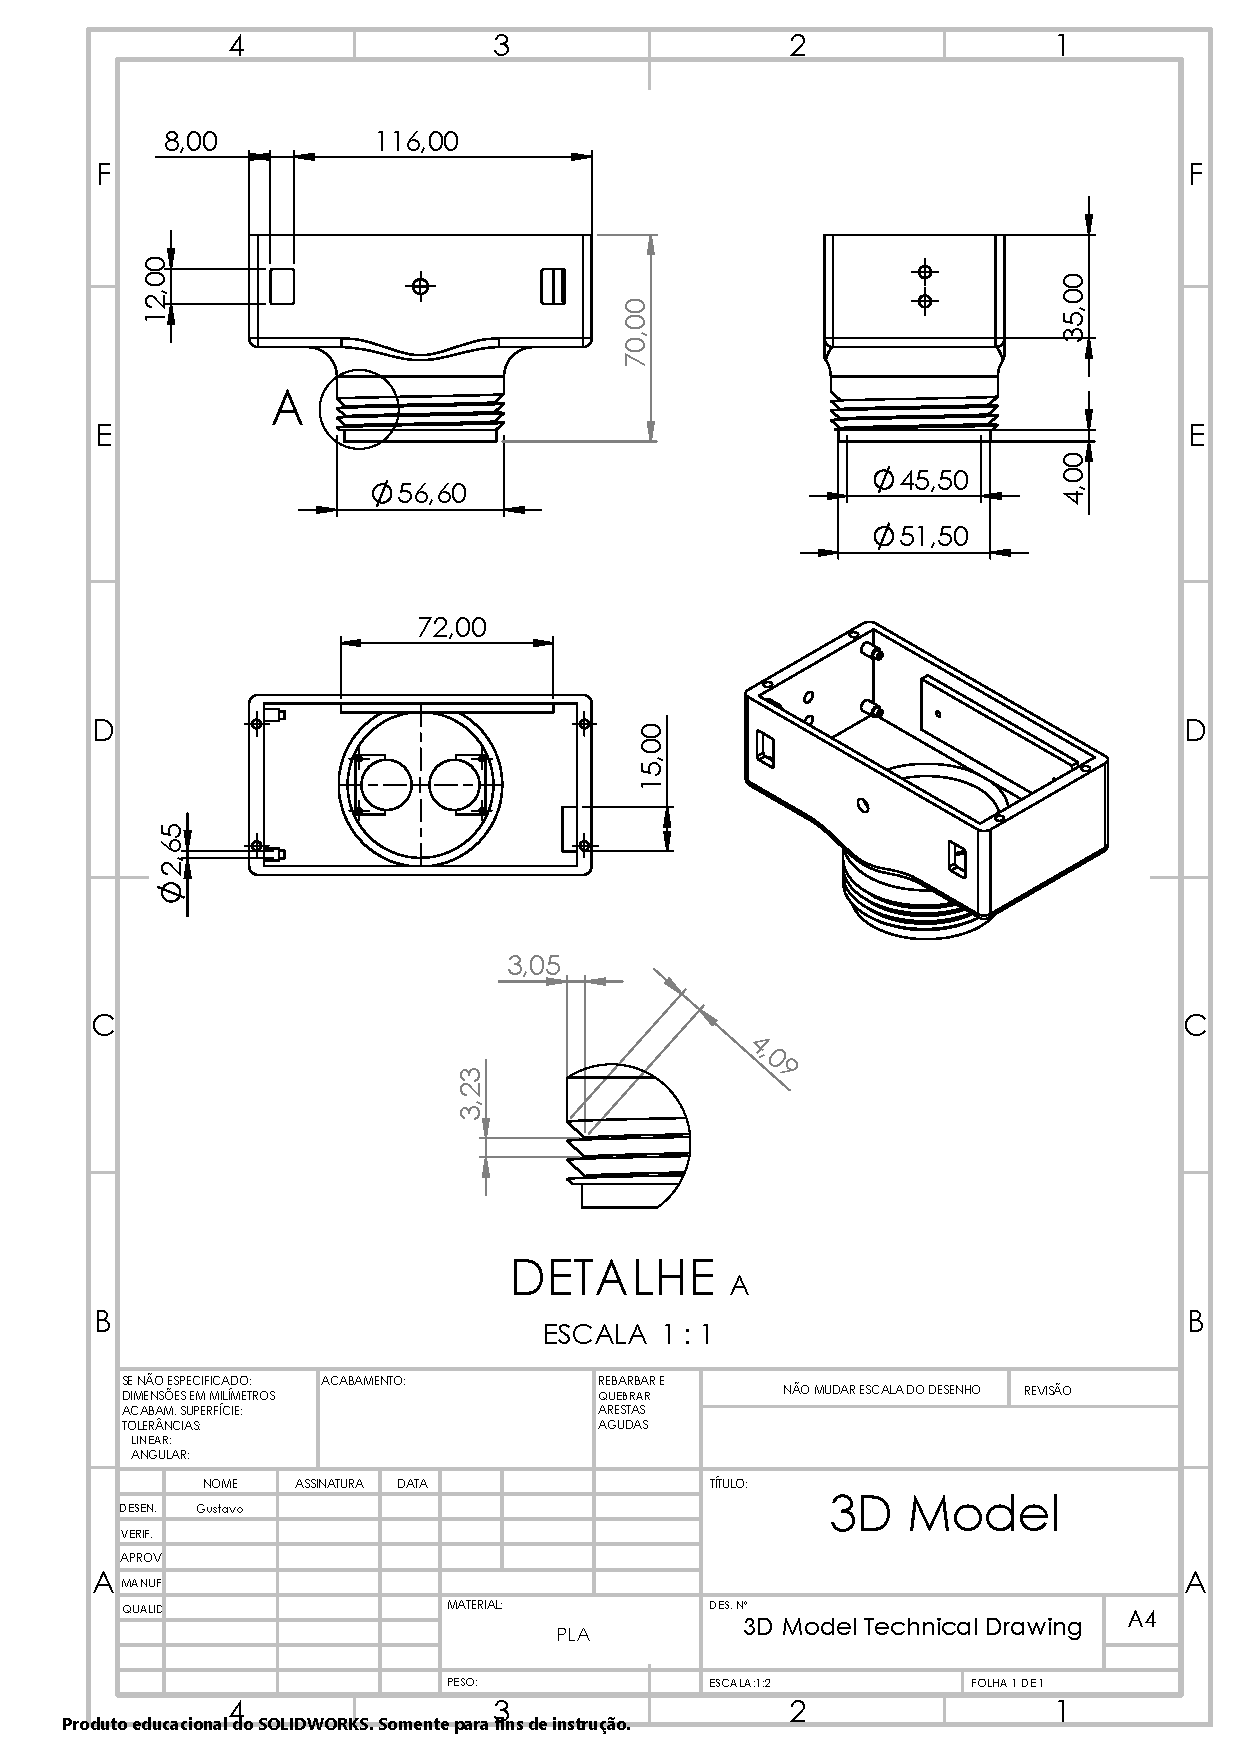
\includegraphics[scale=0.65]{images/Results/3D_Model_Technical_Drawing.PDF}
    \caption{Technical drawing of the 3D printed model.}
    \label{fig:3dModel}
\end{figure}

\begin{figure}[h!]
    \centering
    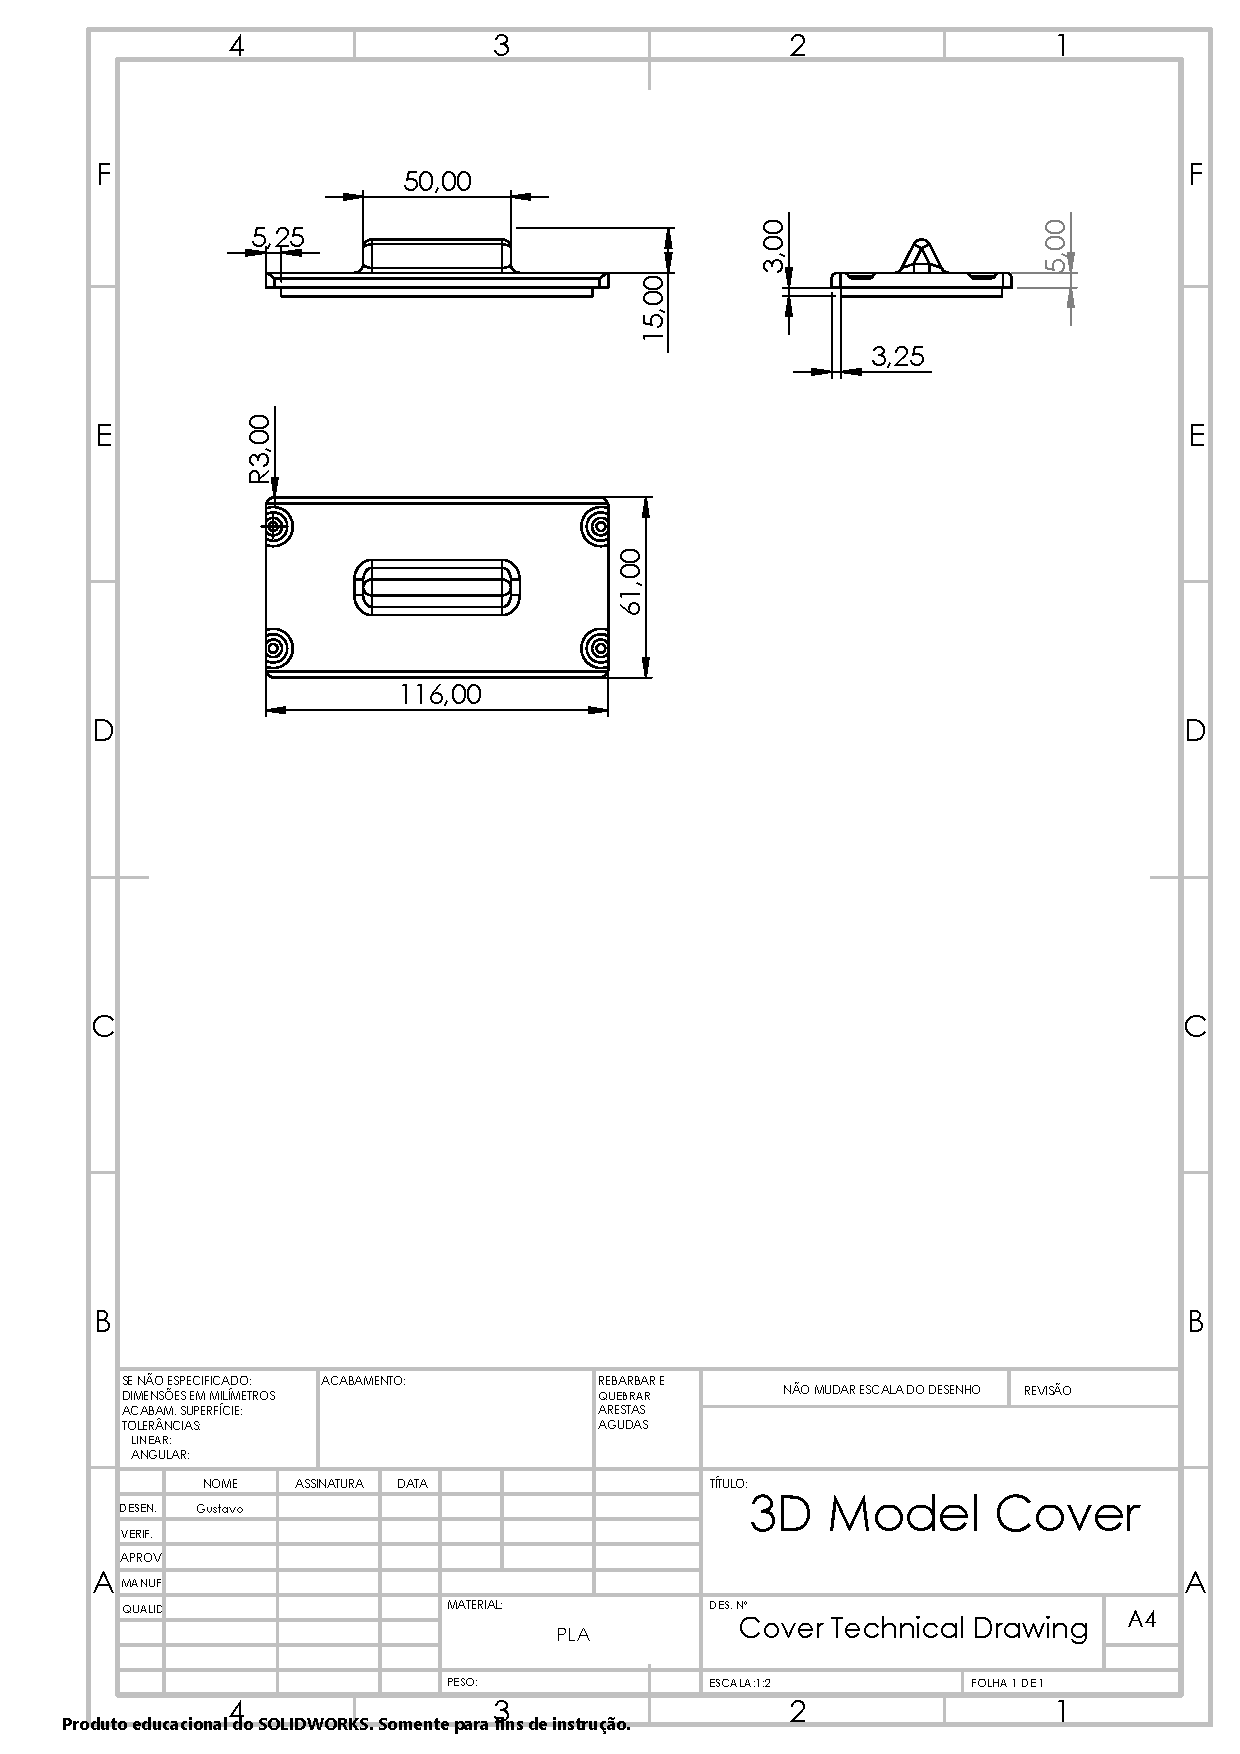
\includegraphics[scale=0.65]{images/Results/3D_Model_Cover_Technical_Drawing.PDF}
    \caption{Technical drawing of the 3D printed cover model.}
    \label{fig:3dModelCover}
\end{figure}

\clearpage
\section{Developed Codes}\label{appendice:code}

\begin{center}
    Link for GitHub, where can be found the files with the codes applied:
\end{center}

\begin{center}
\url{https://github.com/gustavogoncalvescoelho/IoT-Solution-For-Industrial-Washing-Machines}
\end{center}
